\section{Comparison in regard to the existence of Similar Entities}
\label{appendix:similar_entities}
\subsection{AnyBURL and ComplEx on CoDEx-M}

\begin{figure}[H]
\centering
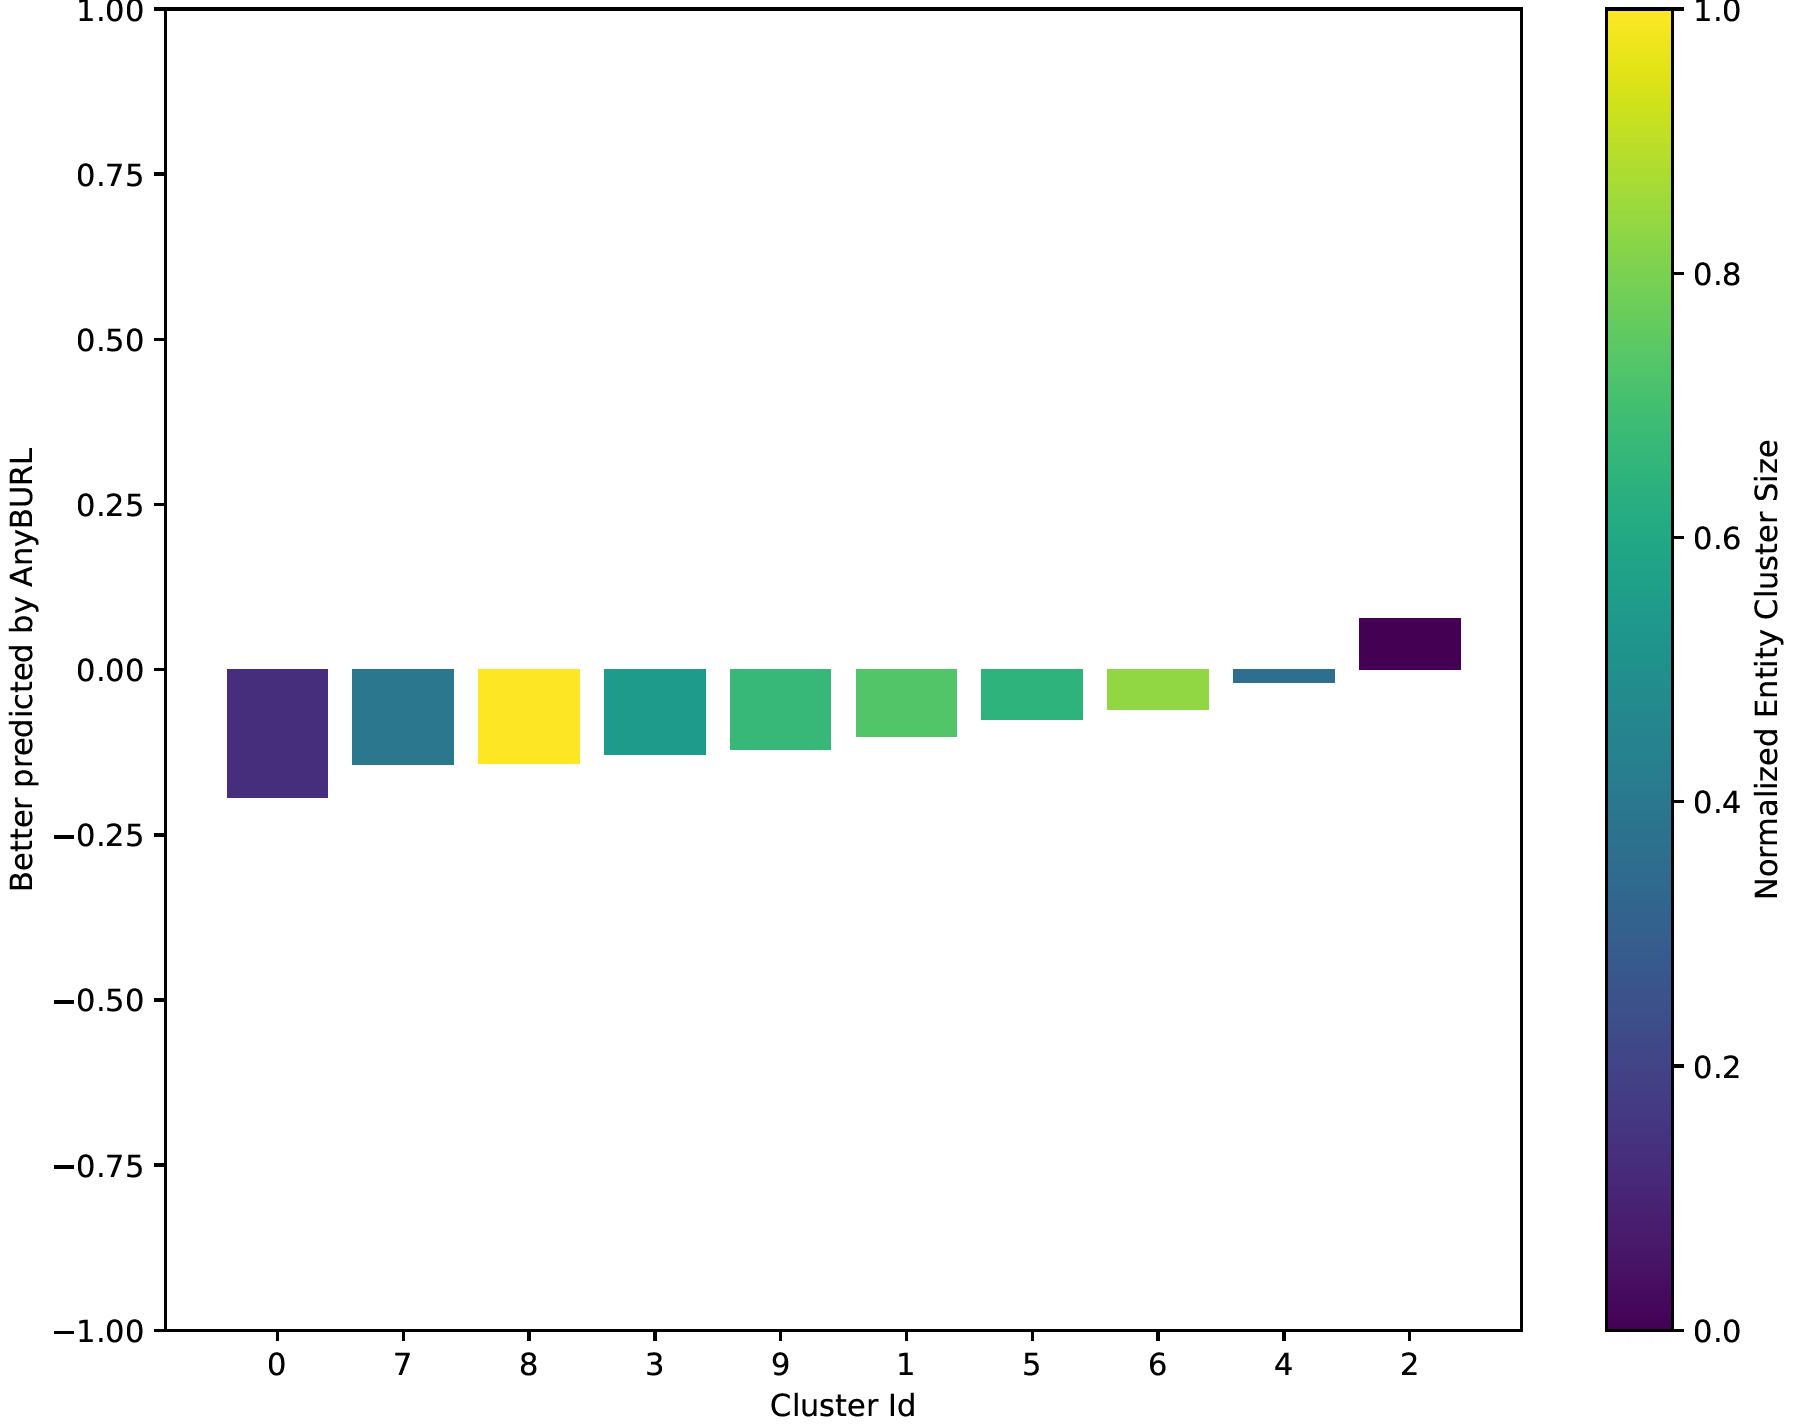
\includegraphics[width=0.7\textwidth]{images/head_cluster_10_anyburl_complex_codex.PNG}
\caption{Comparison of AnyBURL and ComplEx on CoDEx-M in regard to the existence of similar head entities based on K-Means Clustering (k=10)}
\label{fig:head_cluster_10_anyburl_complex_codex}
\end{figure}

\begin{figure}[H]
\centering
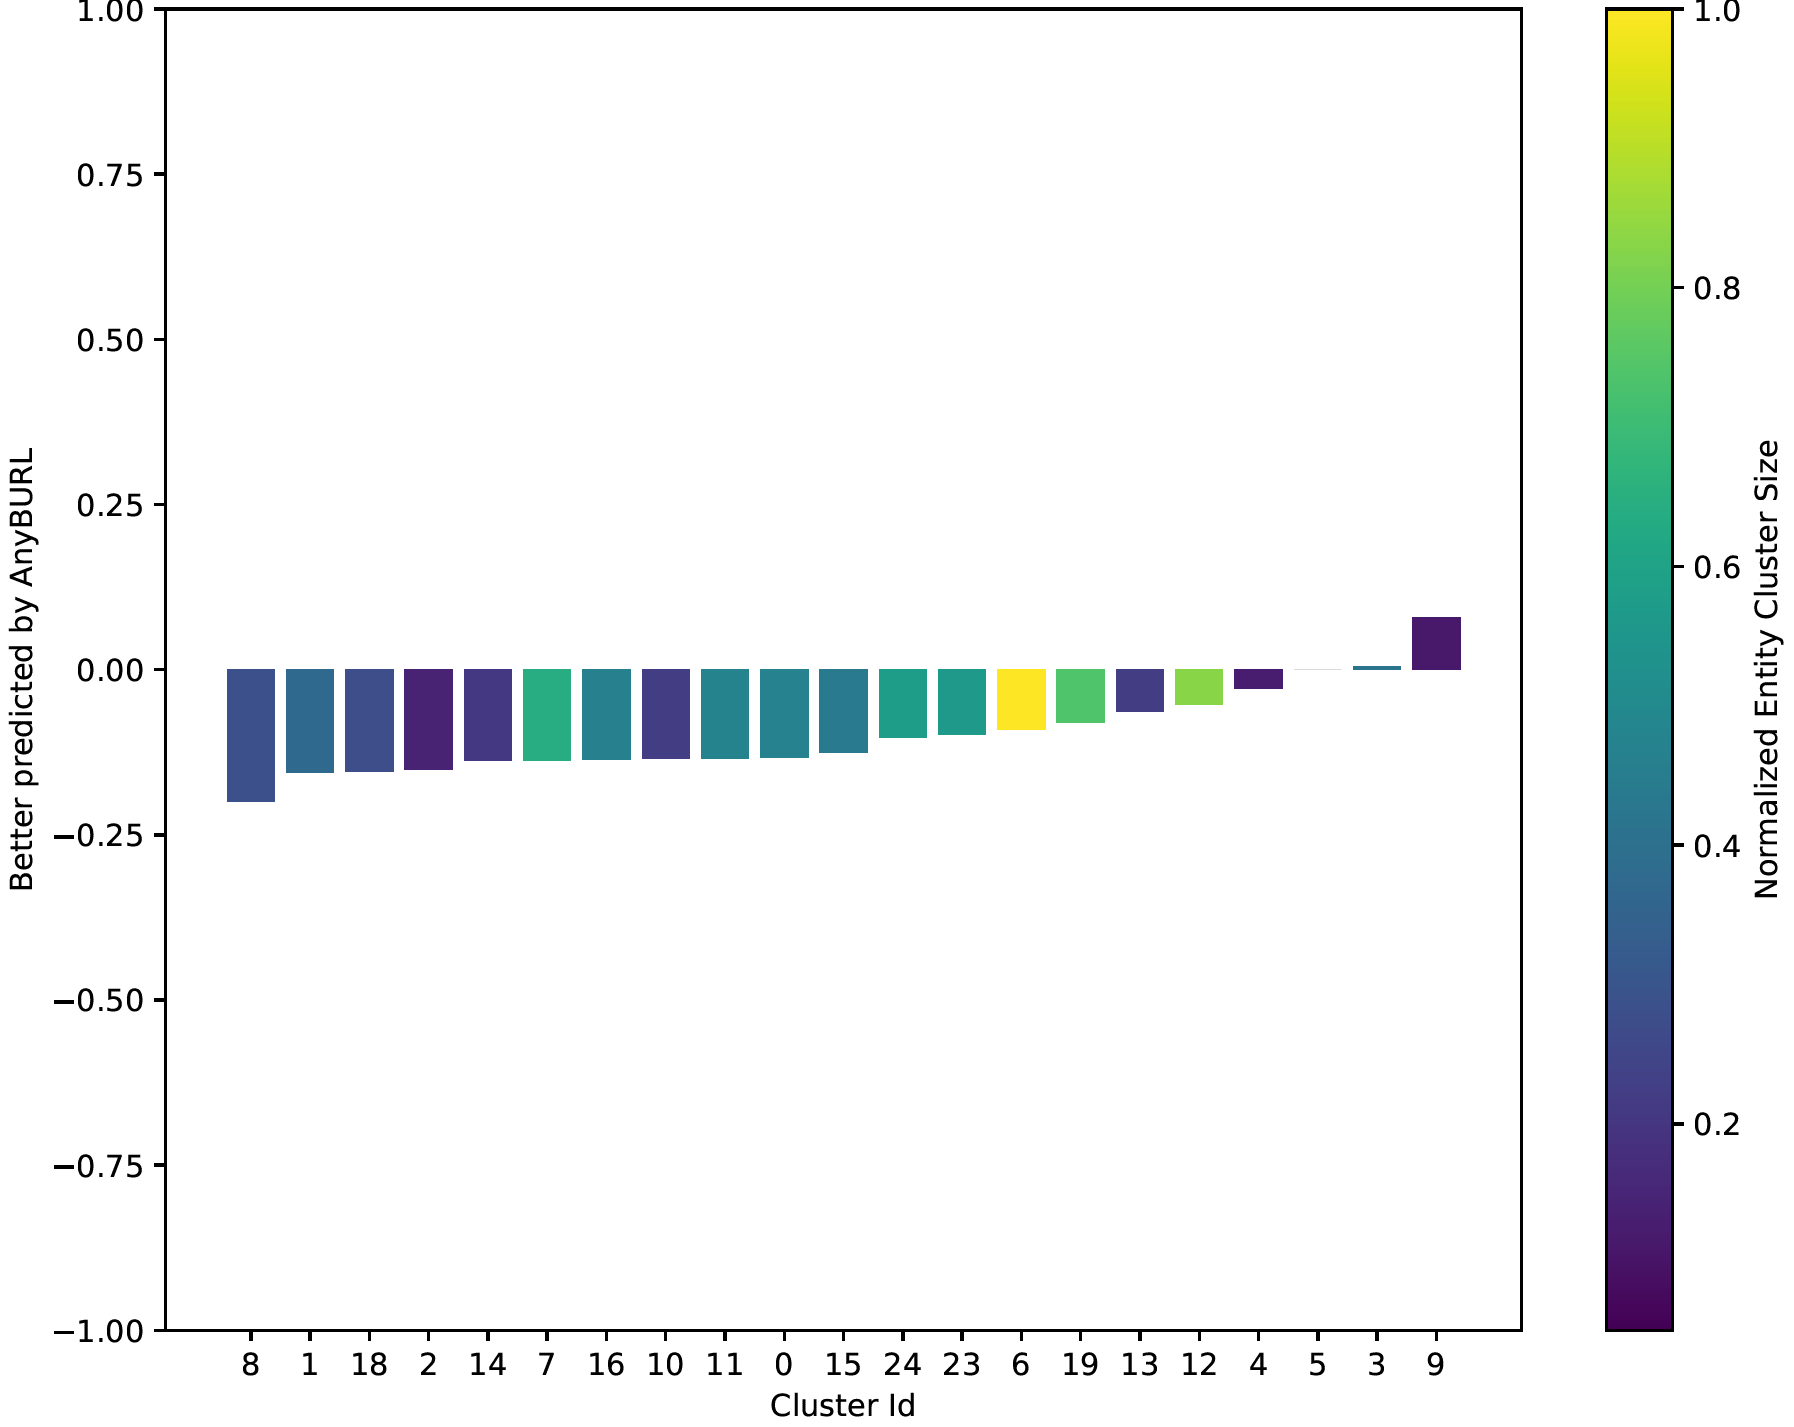
\includegraphics[width=0.7\textwidth]{images/head_cluster_25_anyburl_complex_codex.PNG}
\caption{Comparison of AnyBURL and ComplEx on CoDEx-M in regard to the existence of similar head entities based on K-Means Clustering (k=25)}
\label{fig:head_cluster_25_anyburl_complex_codex}
\end{figure}

\begin{figure}[H]
\centering
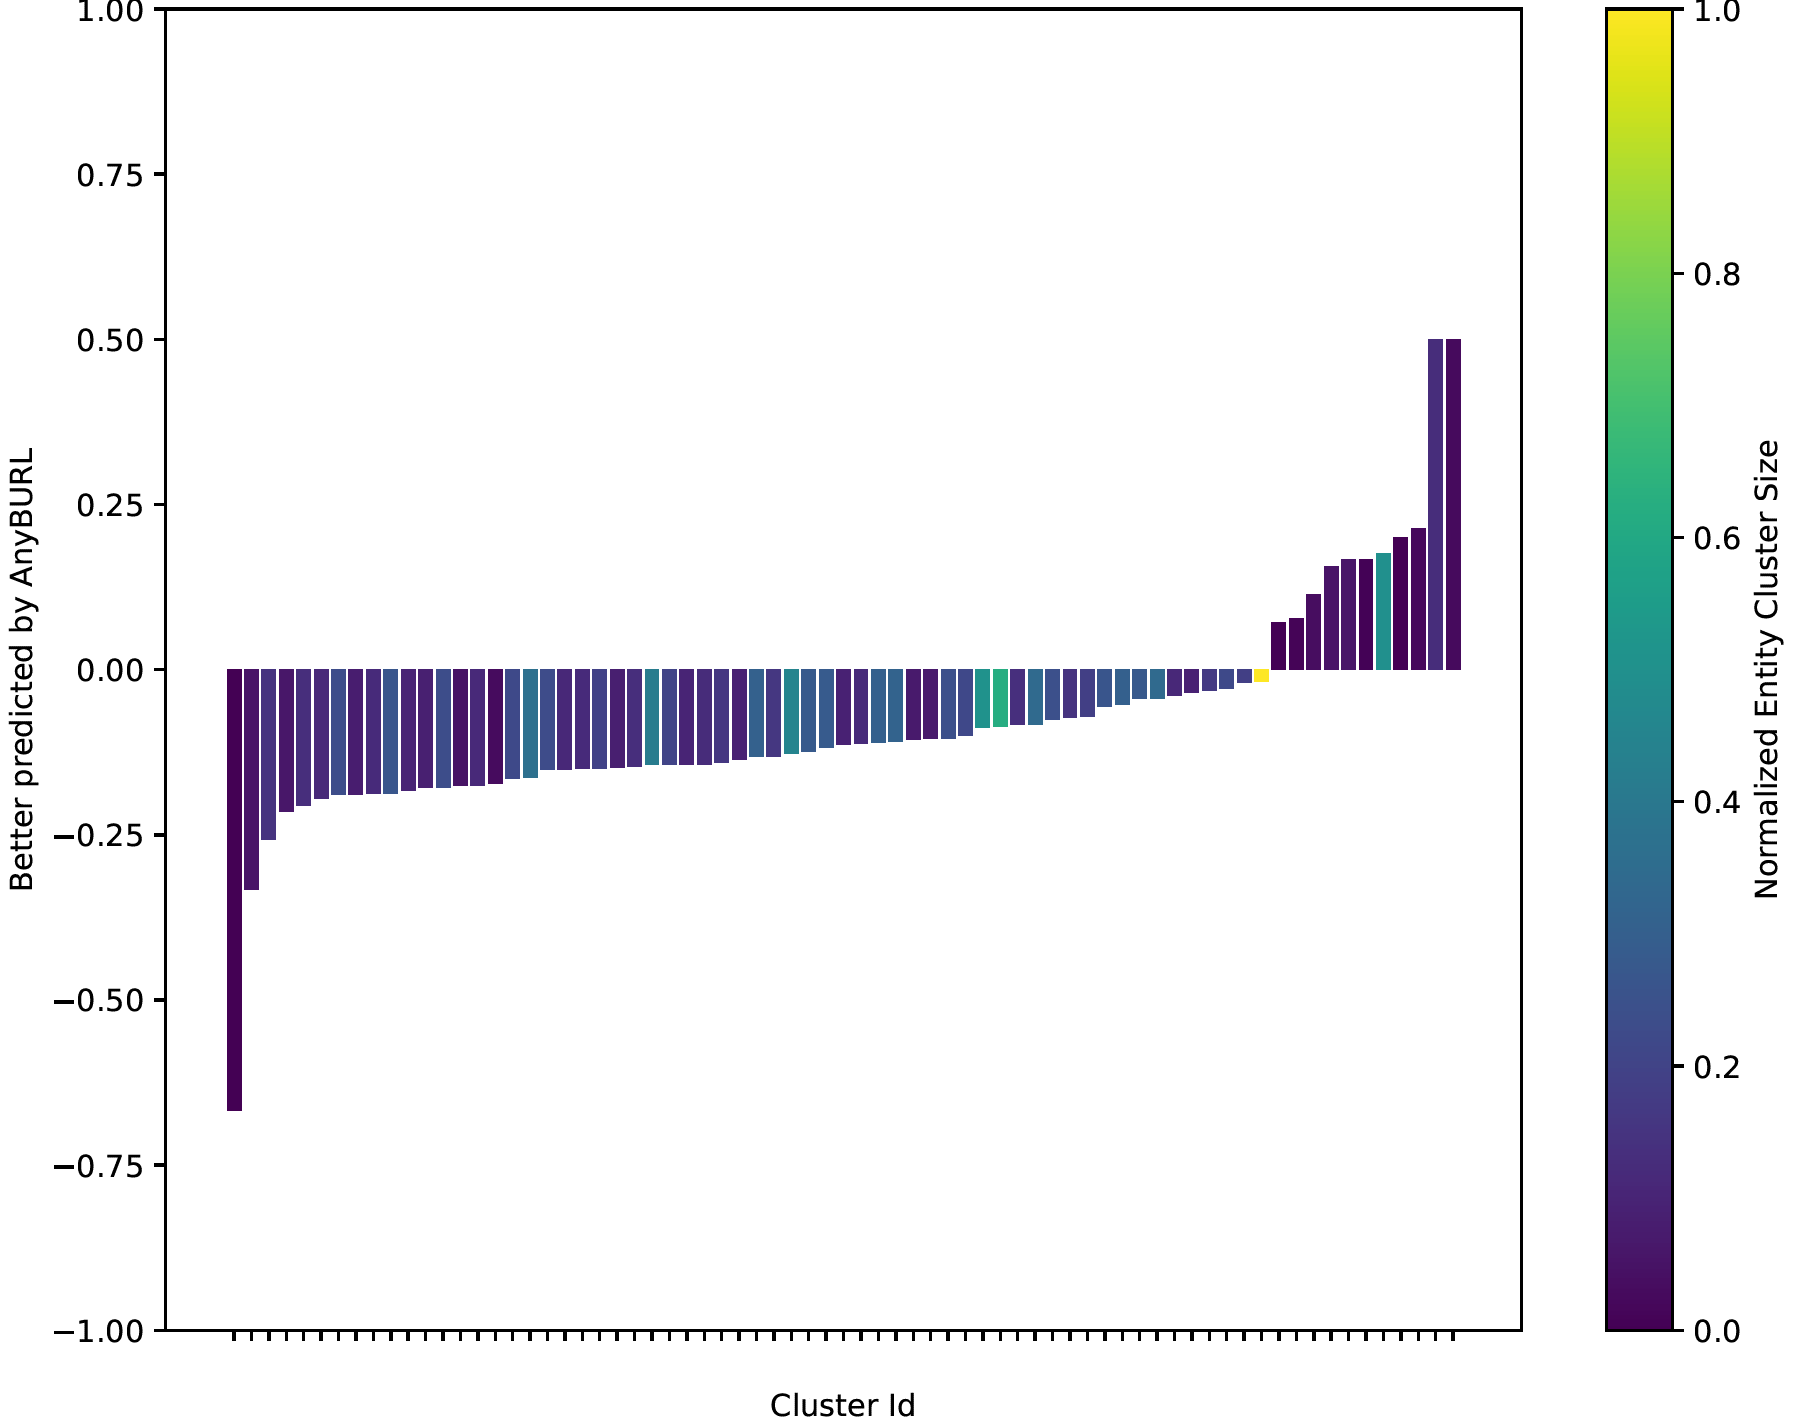
\includegraphics[width=0.7\textwidth]{images/head_cluster_100_anyburl_complex_codex.PNG}
\caption{Comparison of AnyBURL and ComplEx on CoDEx-M in regard to the existence of similar head entities based on K-Means Clustering (k=100)}
\label{fig:head_cluster_100_anyburl_complex_codex}
\end{figure}

\begin{figure}[H]
\centering
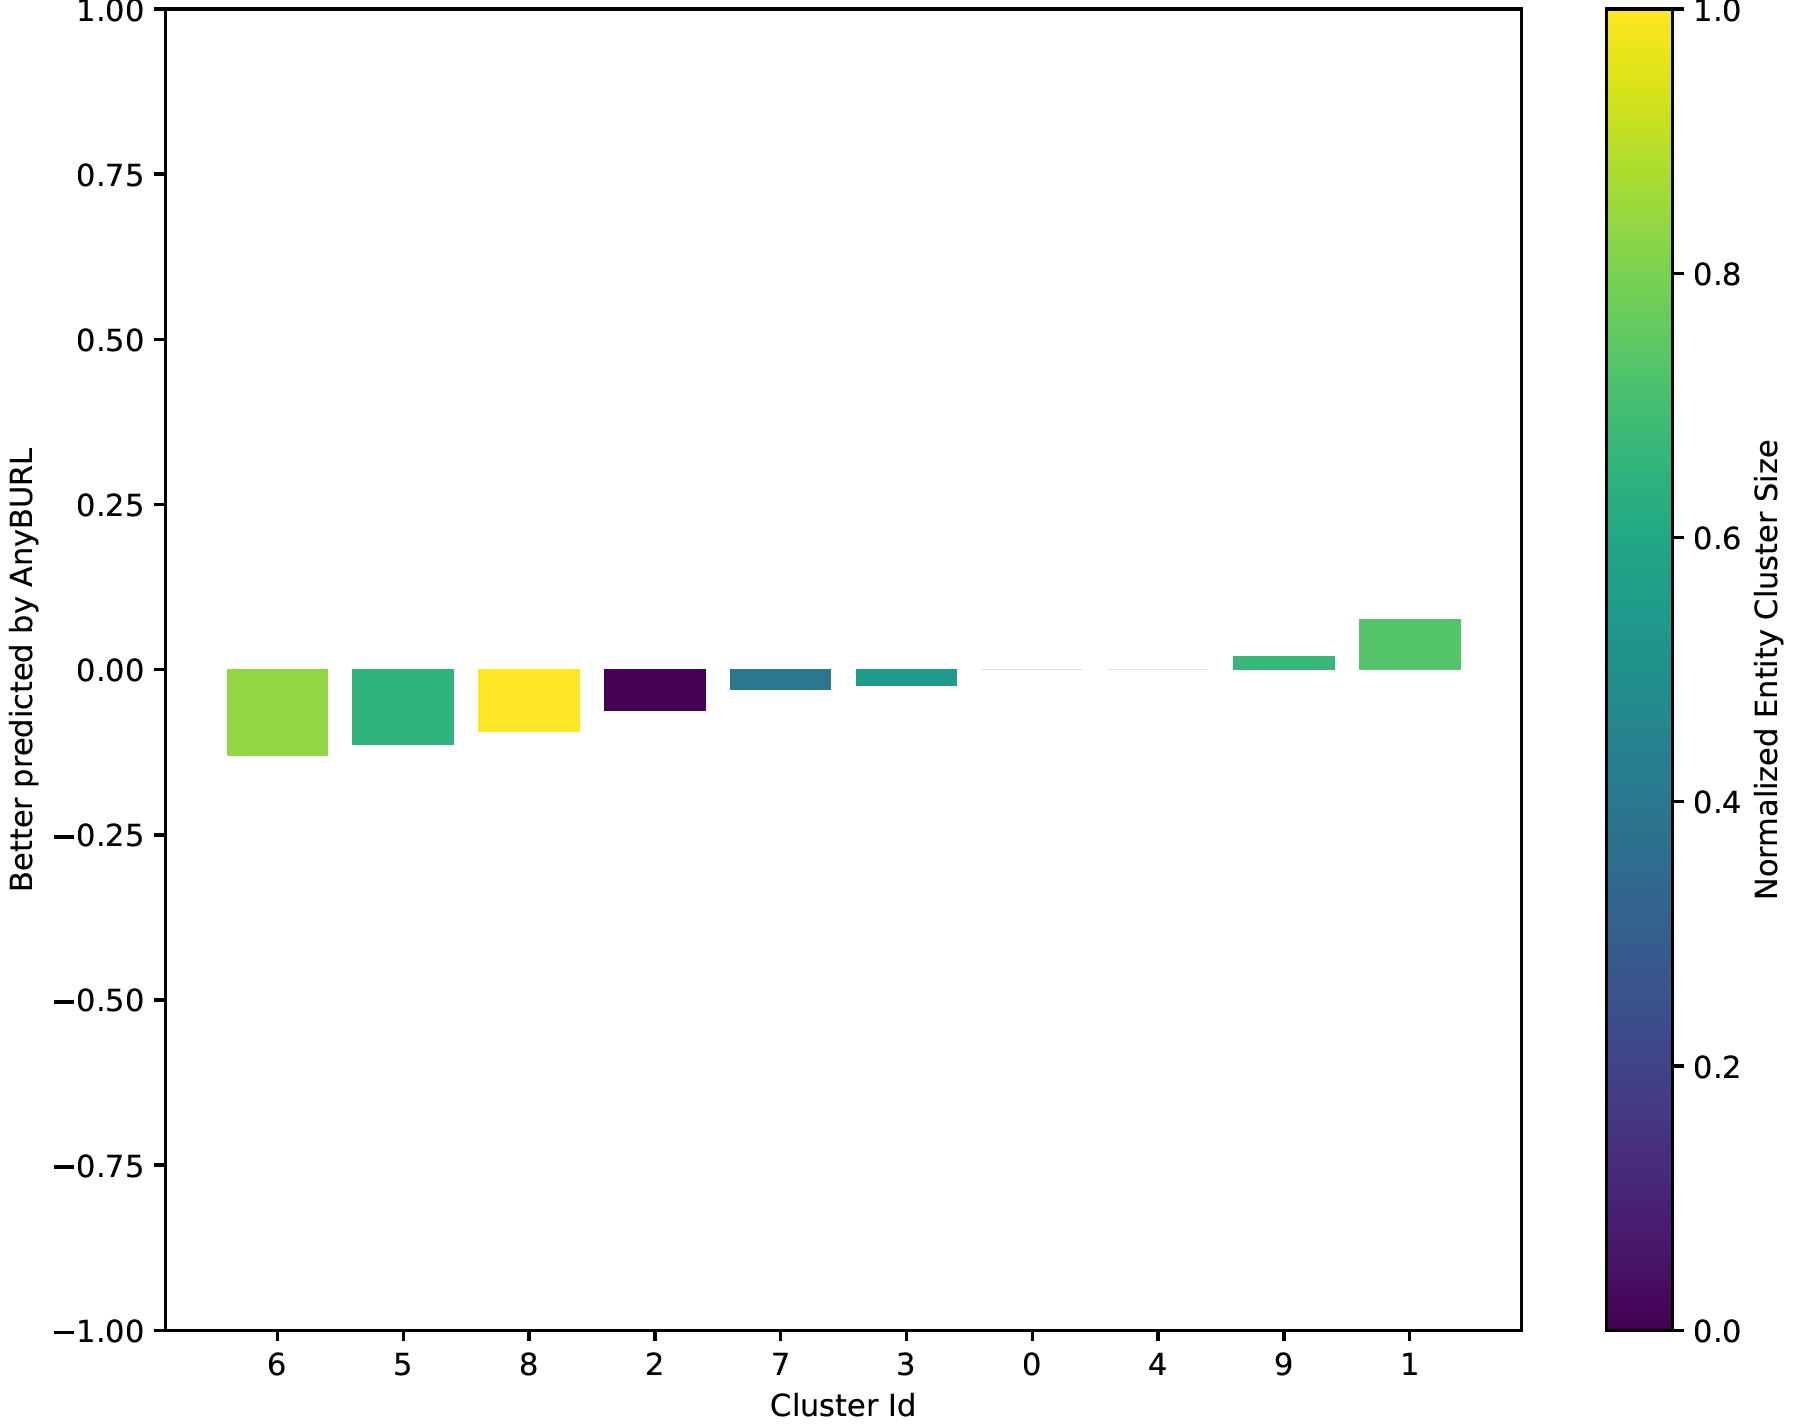
\includegraphics[width=0.7\textwidth]{images/tail_cluster_10_anyburl_complex_codex.PNG}
\caption{Comparison of AnyBURL and ComplEx on CoDEx-M in regard to the existence of similar tail entities based on K-Means Clustering (k=10)}
\label{fig:tail_cluster_10_anyburl_complex_codex}
\end{figure}

\begin{figure}[H]
\centering
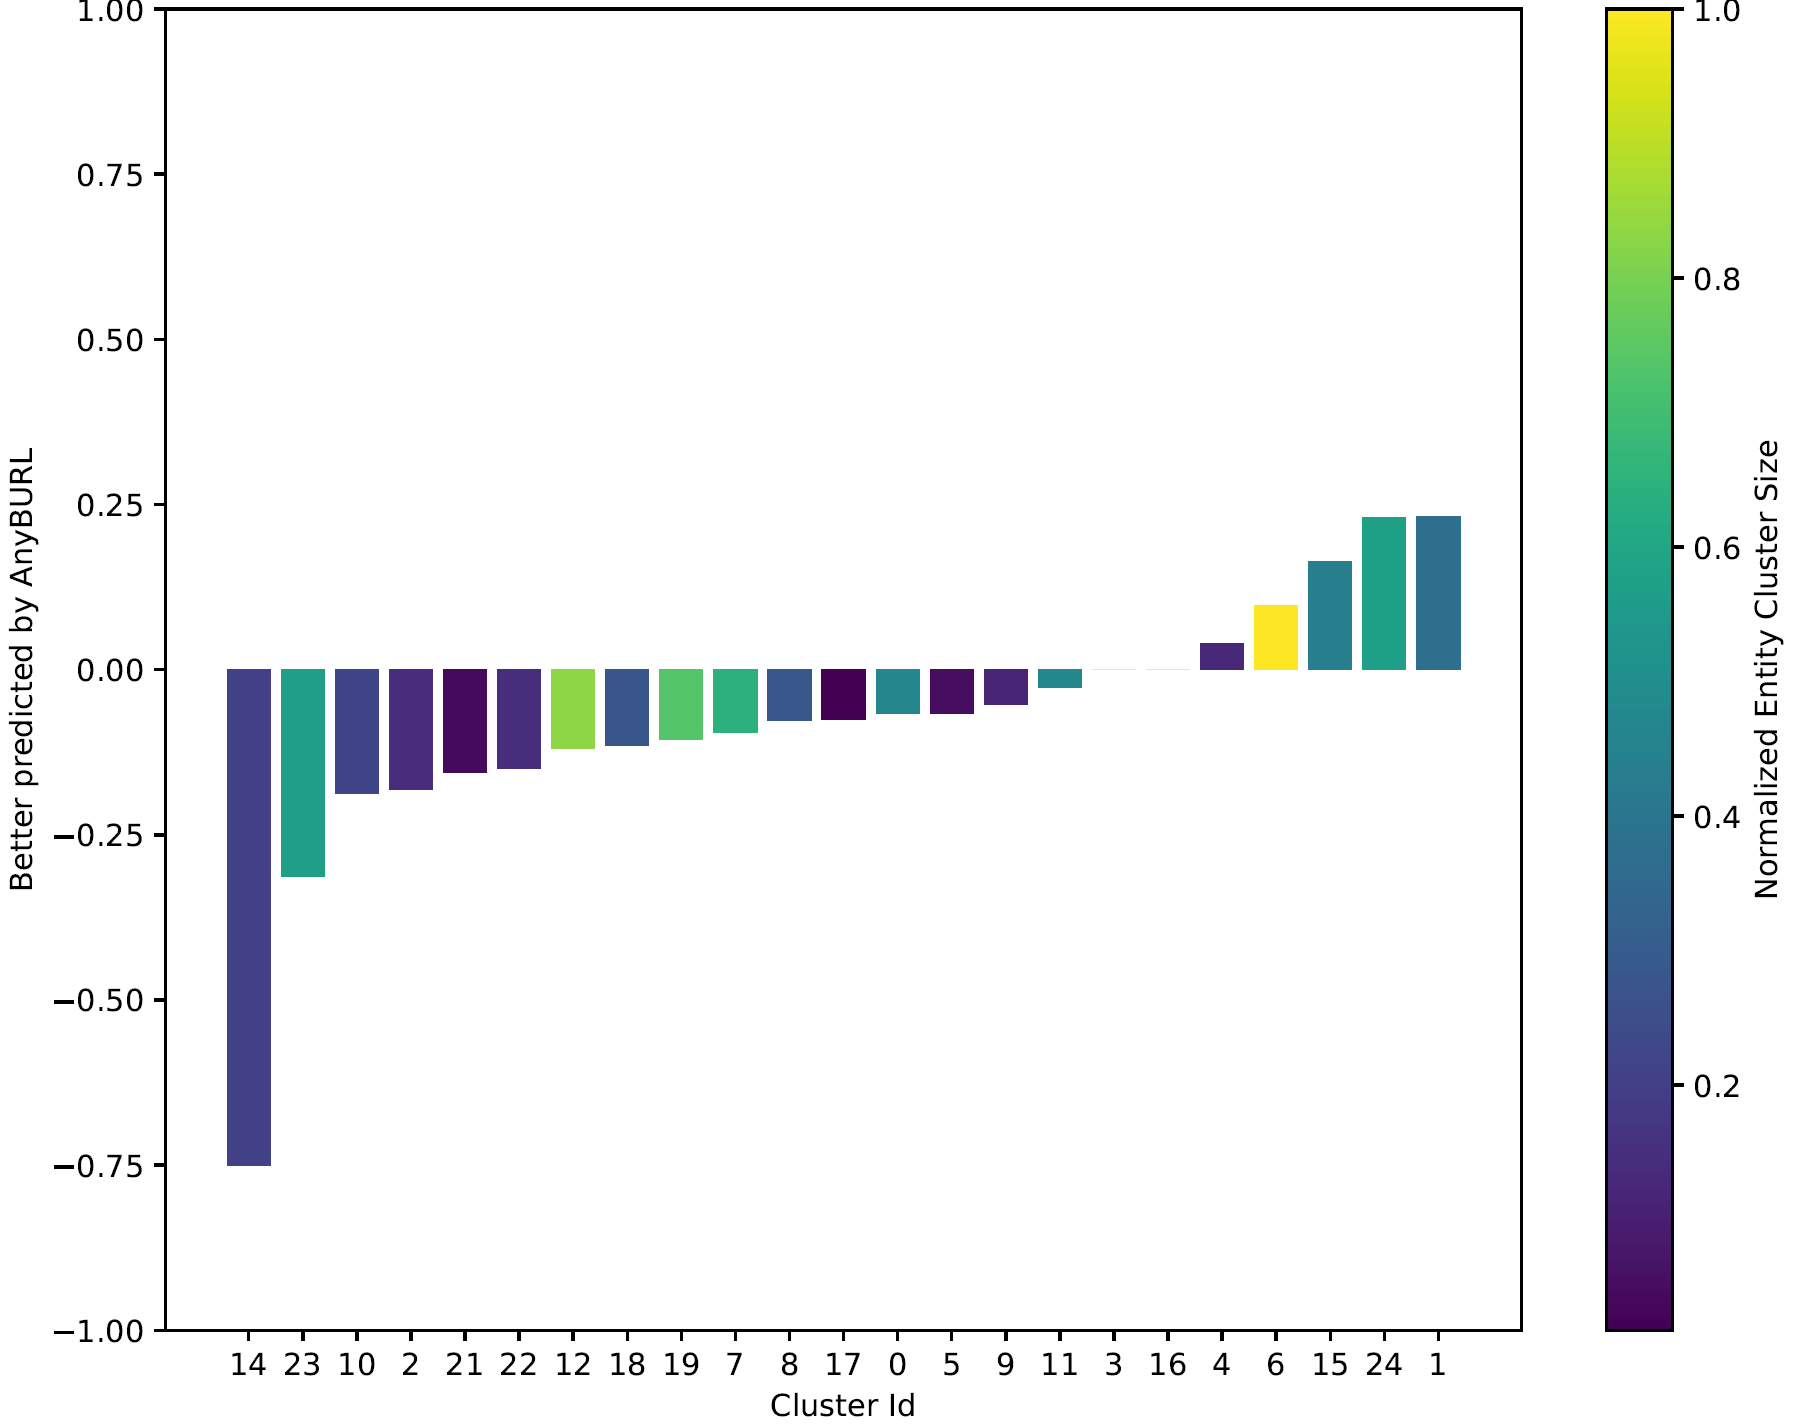
\includegraphics[width=0.7\textwidth]{images/tail_cluster_25_anyburl_complex_codex.PNG}
\caption{Comparison of AnyBURL and ComplEx on CoDEx-M in regard to the existence of similar tail entities based on K-Means Clustering (k=25)}
\label{fig:tail_cluster_25_anyburl_complex_codex}
\end{figure}



\subsection{AnyBURL and ConvE on CoDEx-M}

\begin{figure}[H]
\centering
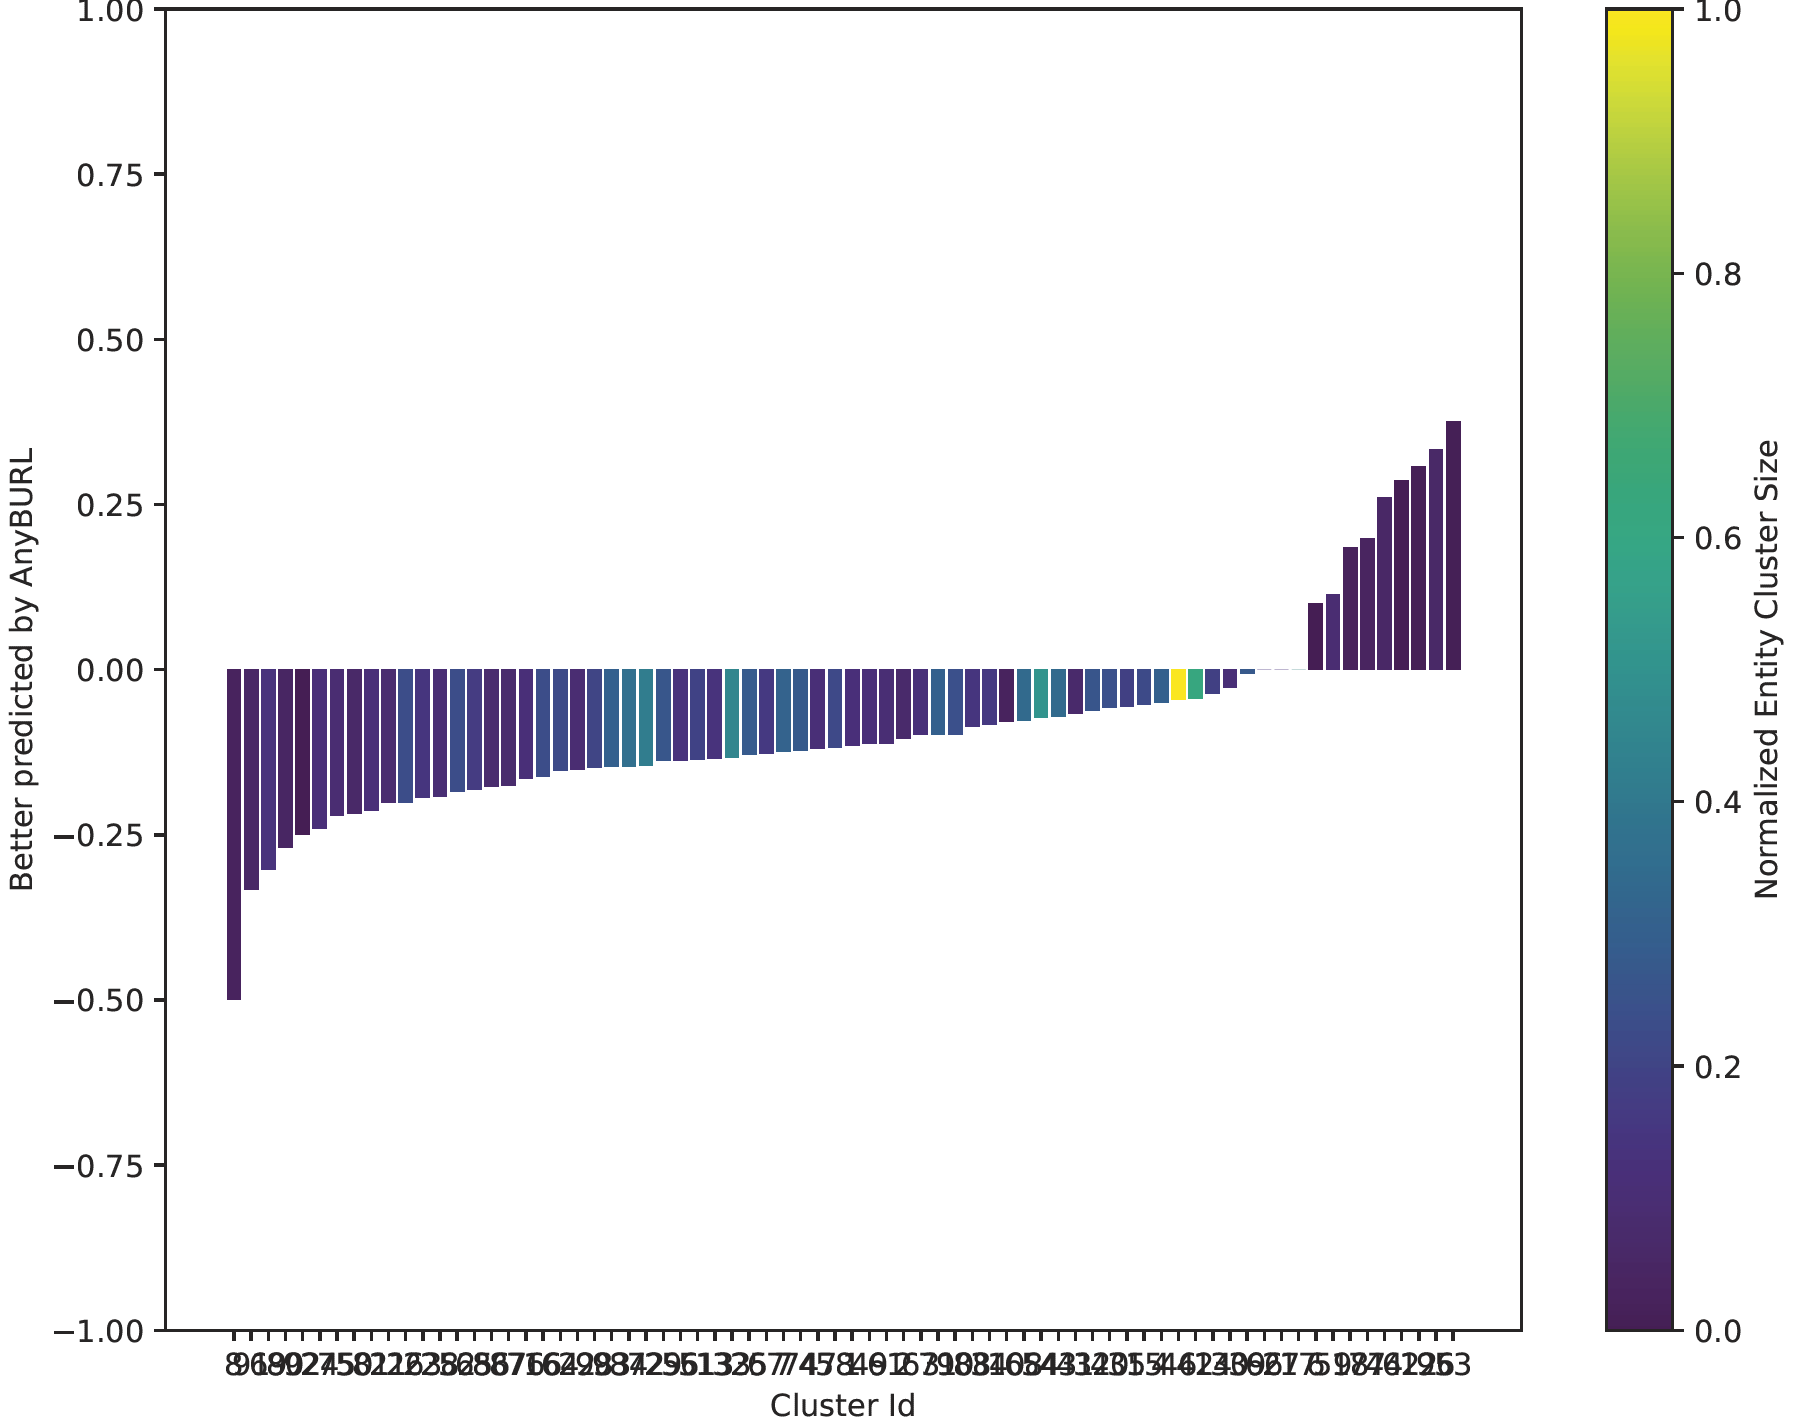
\includegraphics[width=0.7\textwidth]{images/head_cluster_100_anyburl_conve_codex.PNG}
\caption{Comparison of AnyBURL and ConvE on CoDEx-M in regard to the existence of similar head entities based on K-Means Clustering (k=100)}
\label{fig:head_cluster_100_anyburl_conve_codex}
\end{figure}


\subsection{AnyBURL and RESCAL on CoDEx-M}

\begin{figure}[H]
\centering
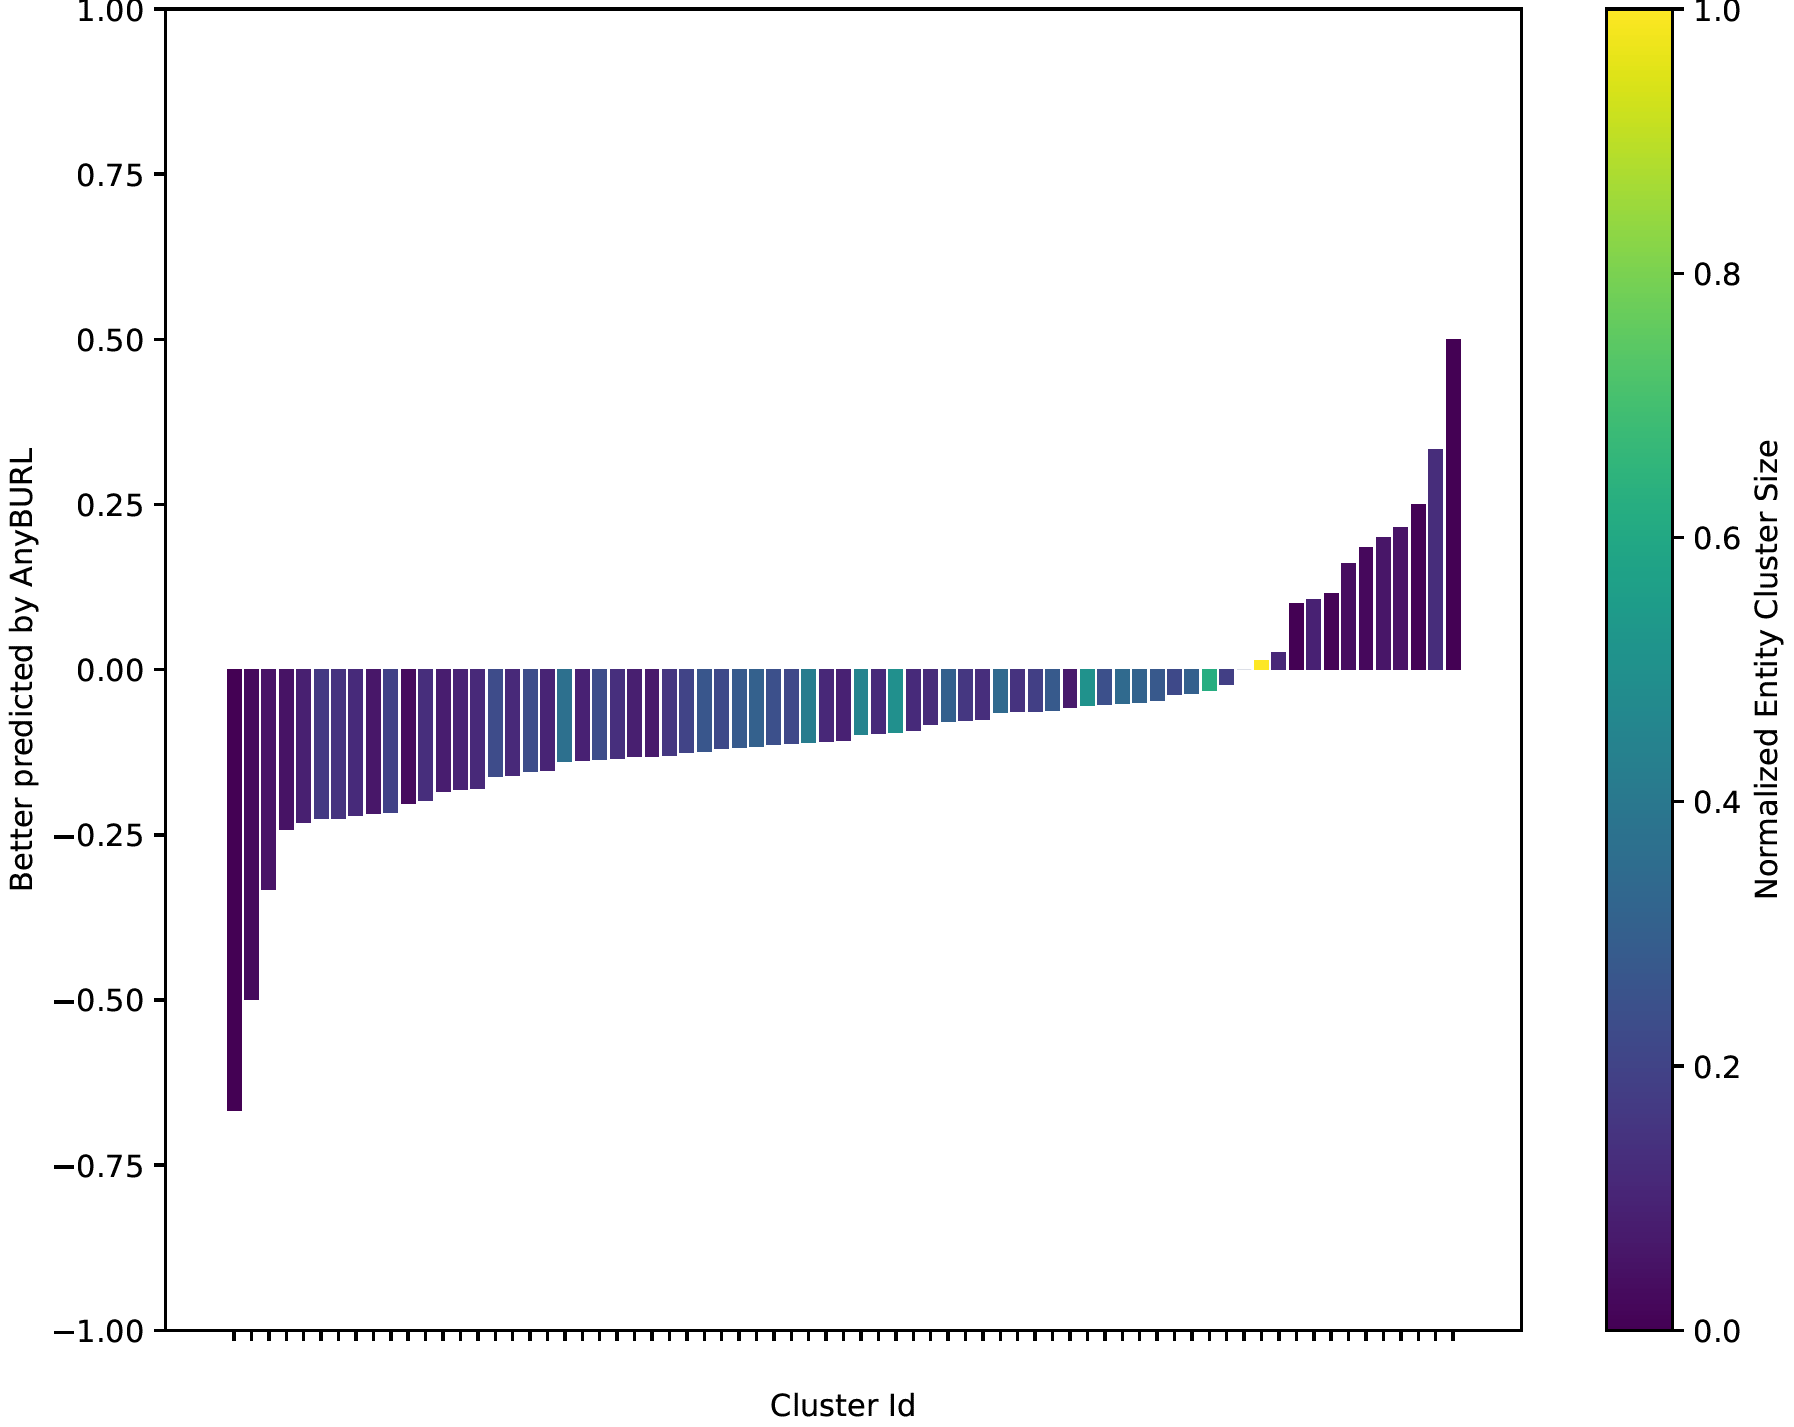
\includegraphics[width=0.7\textwidth]{images/head_cluster_100_anyburl_rescal_codex.PNG}
\caption{Comparison of AnyBURL and ConvE on CoDEx-M in regard to the existence of similar head entities based on K-Means Clustering (k=100)}
\label{fig:head_cluster_100_anyburl_rescal_codex}
\end{figure}

\subsection{AnyBURL and ComplEx on FB15k-237}

\begin{figure}[H]
\centering
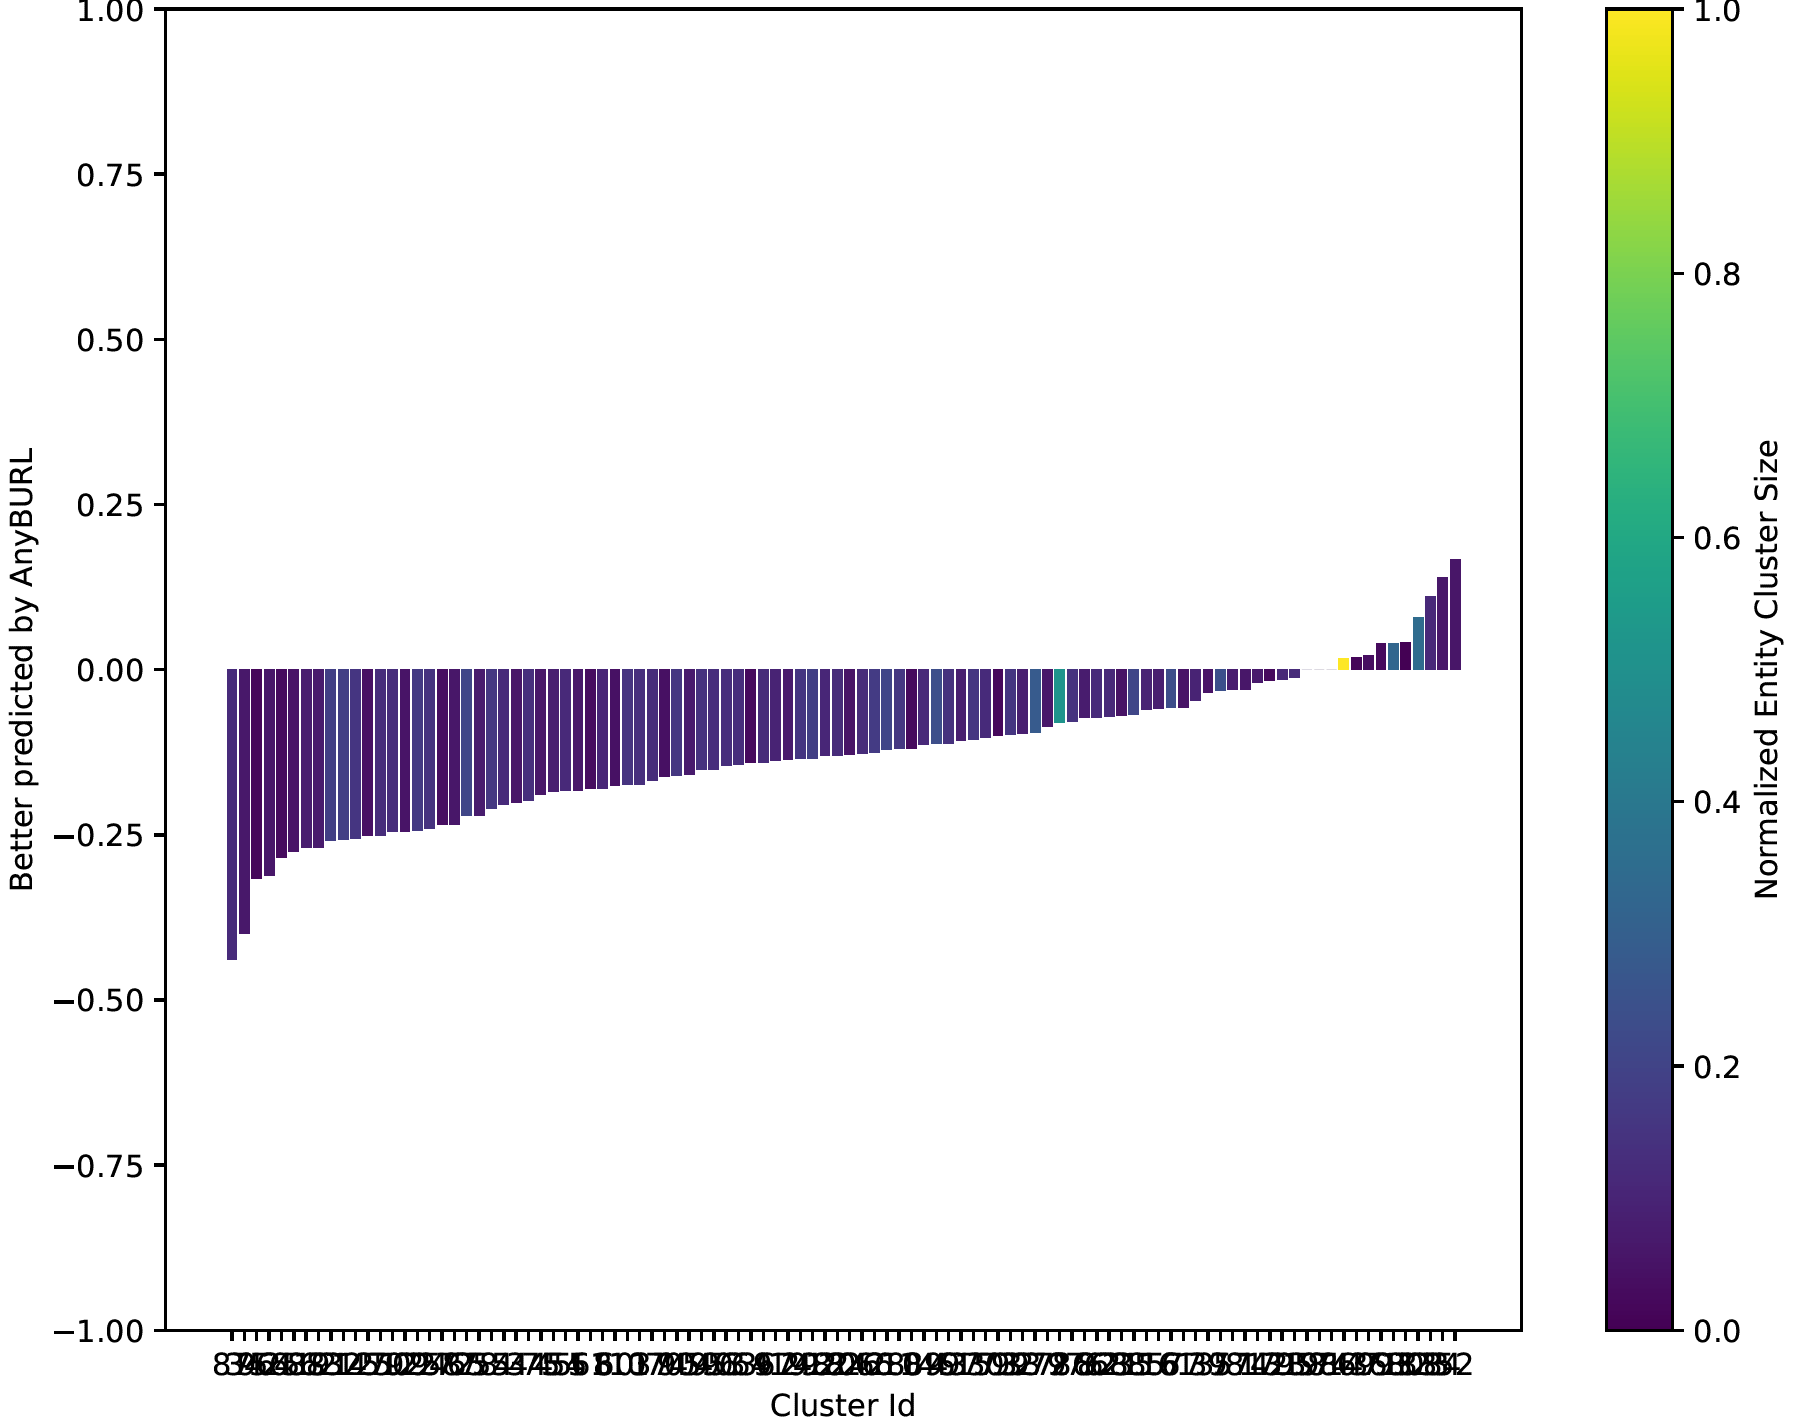
\includegraphics[width=0.7\textwidth]{images/head_cluster_100_anyburl_complex_fb15k.PNG}
\caption{Comparison of AnyBURL and ComplEx on FB15k-237 in regard to the existence of similar head entities based on K-Means Clustering (k=100)}
\label{fig:head_cluster_100_anyburl_complex_fb15k}
\end{figure}

\subsection{AnyBURL and ConvE on FB15k-237}

\begin{figure}[H]
\centering
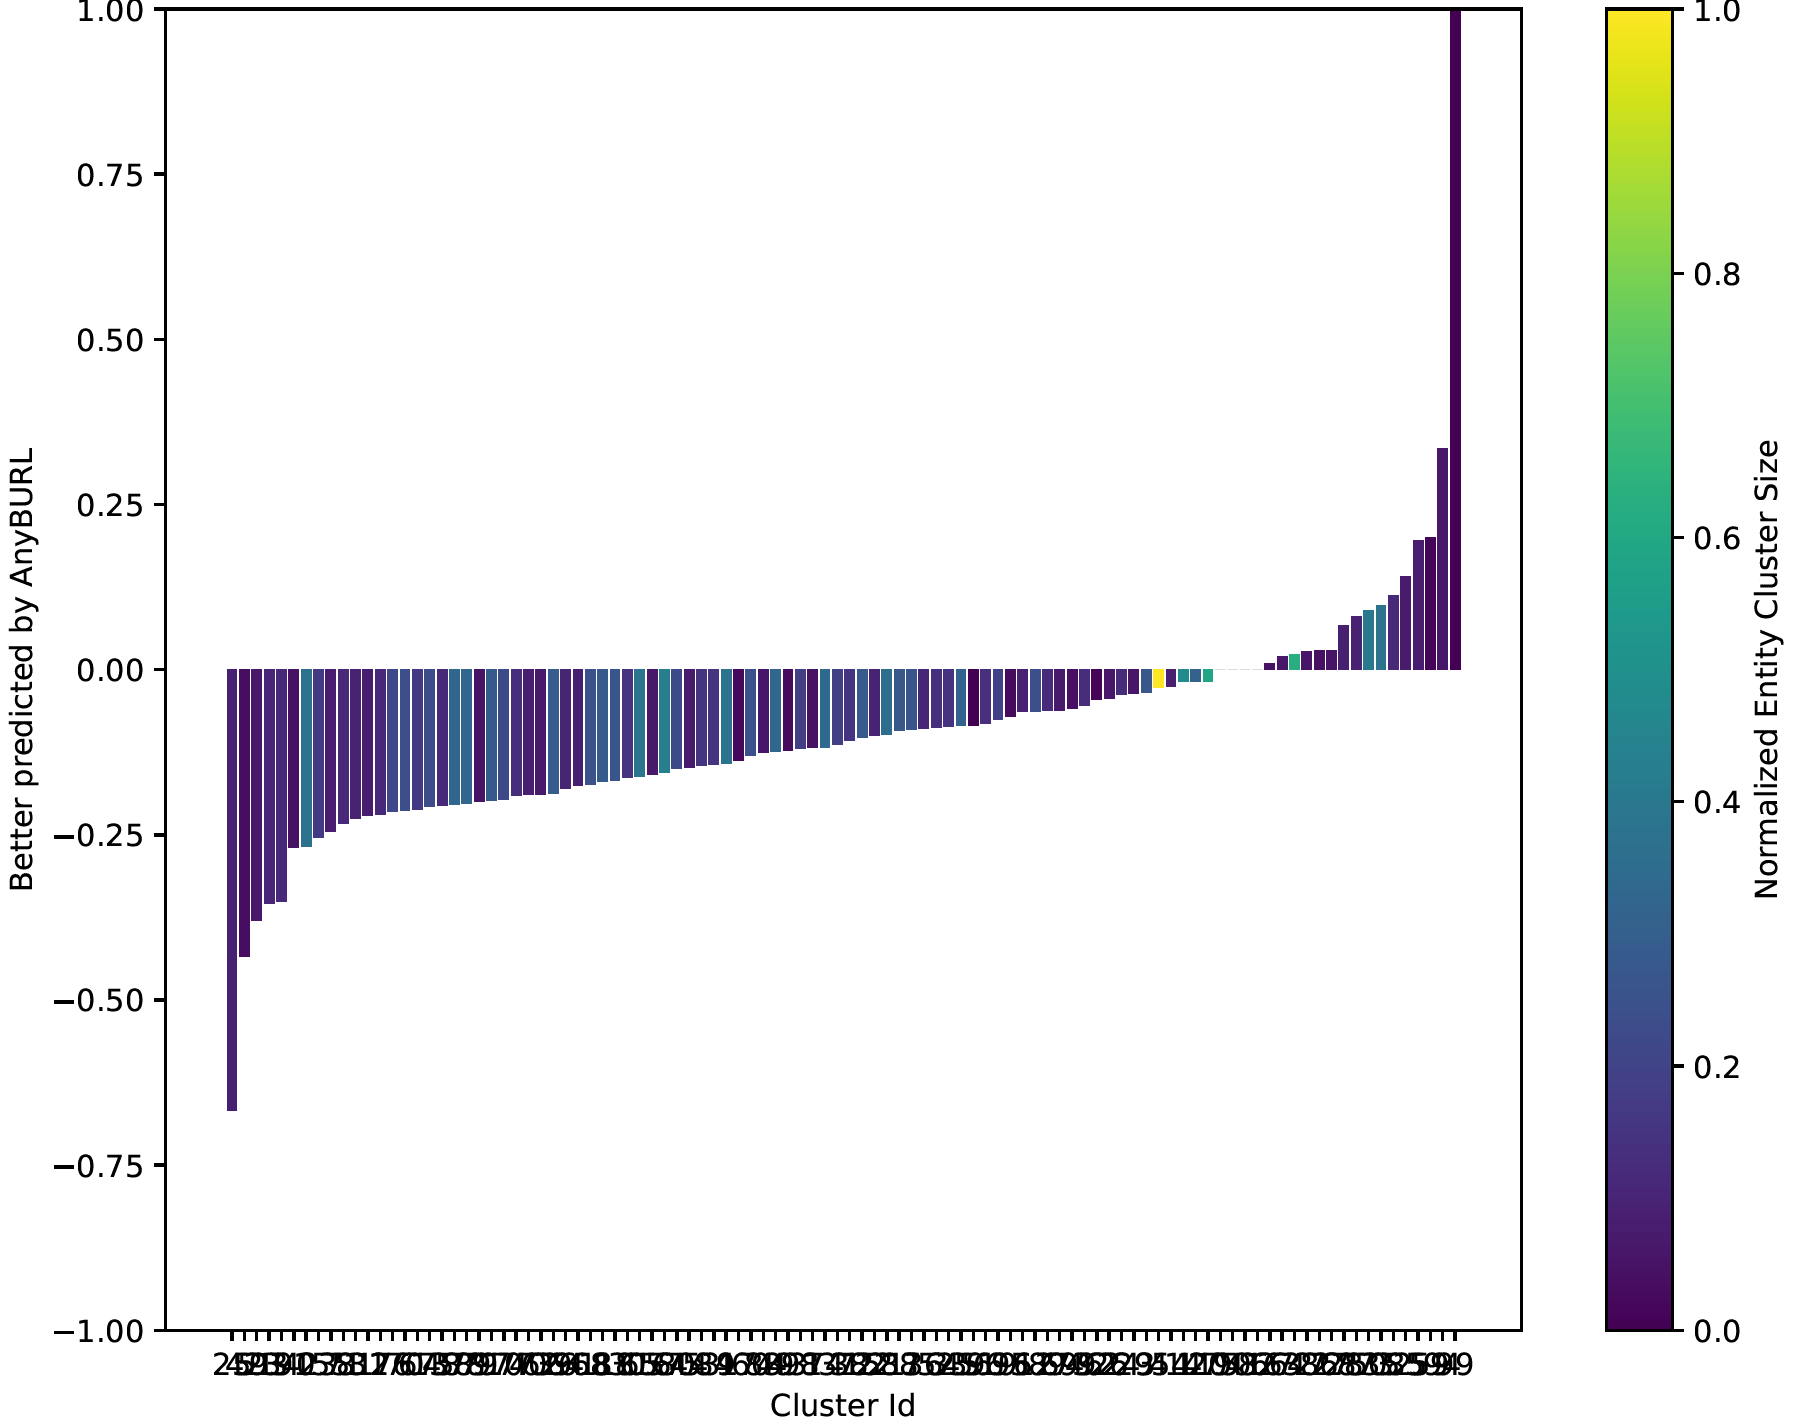
\includegraphics[width=0.7\textwidth]{images/head_cluster_100_anyburl_conve_fb15k.PNG}
\caption{Comparison of AnyBURL and ConvE on FB15k-237 in regard to the existence of similar head entities based on K-Means Clustering (k=100)}
\label{fig:head_cluster_100_anyburl_conve_fb15k}
\end{figure}

\begin{figure}[H]
\centering
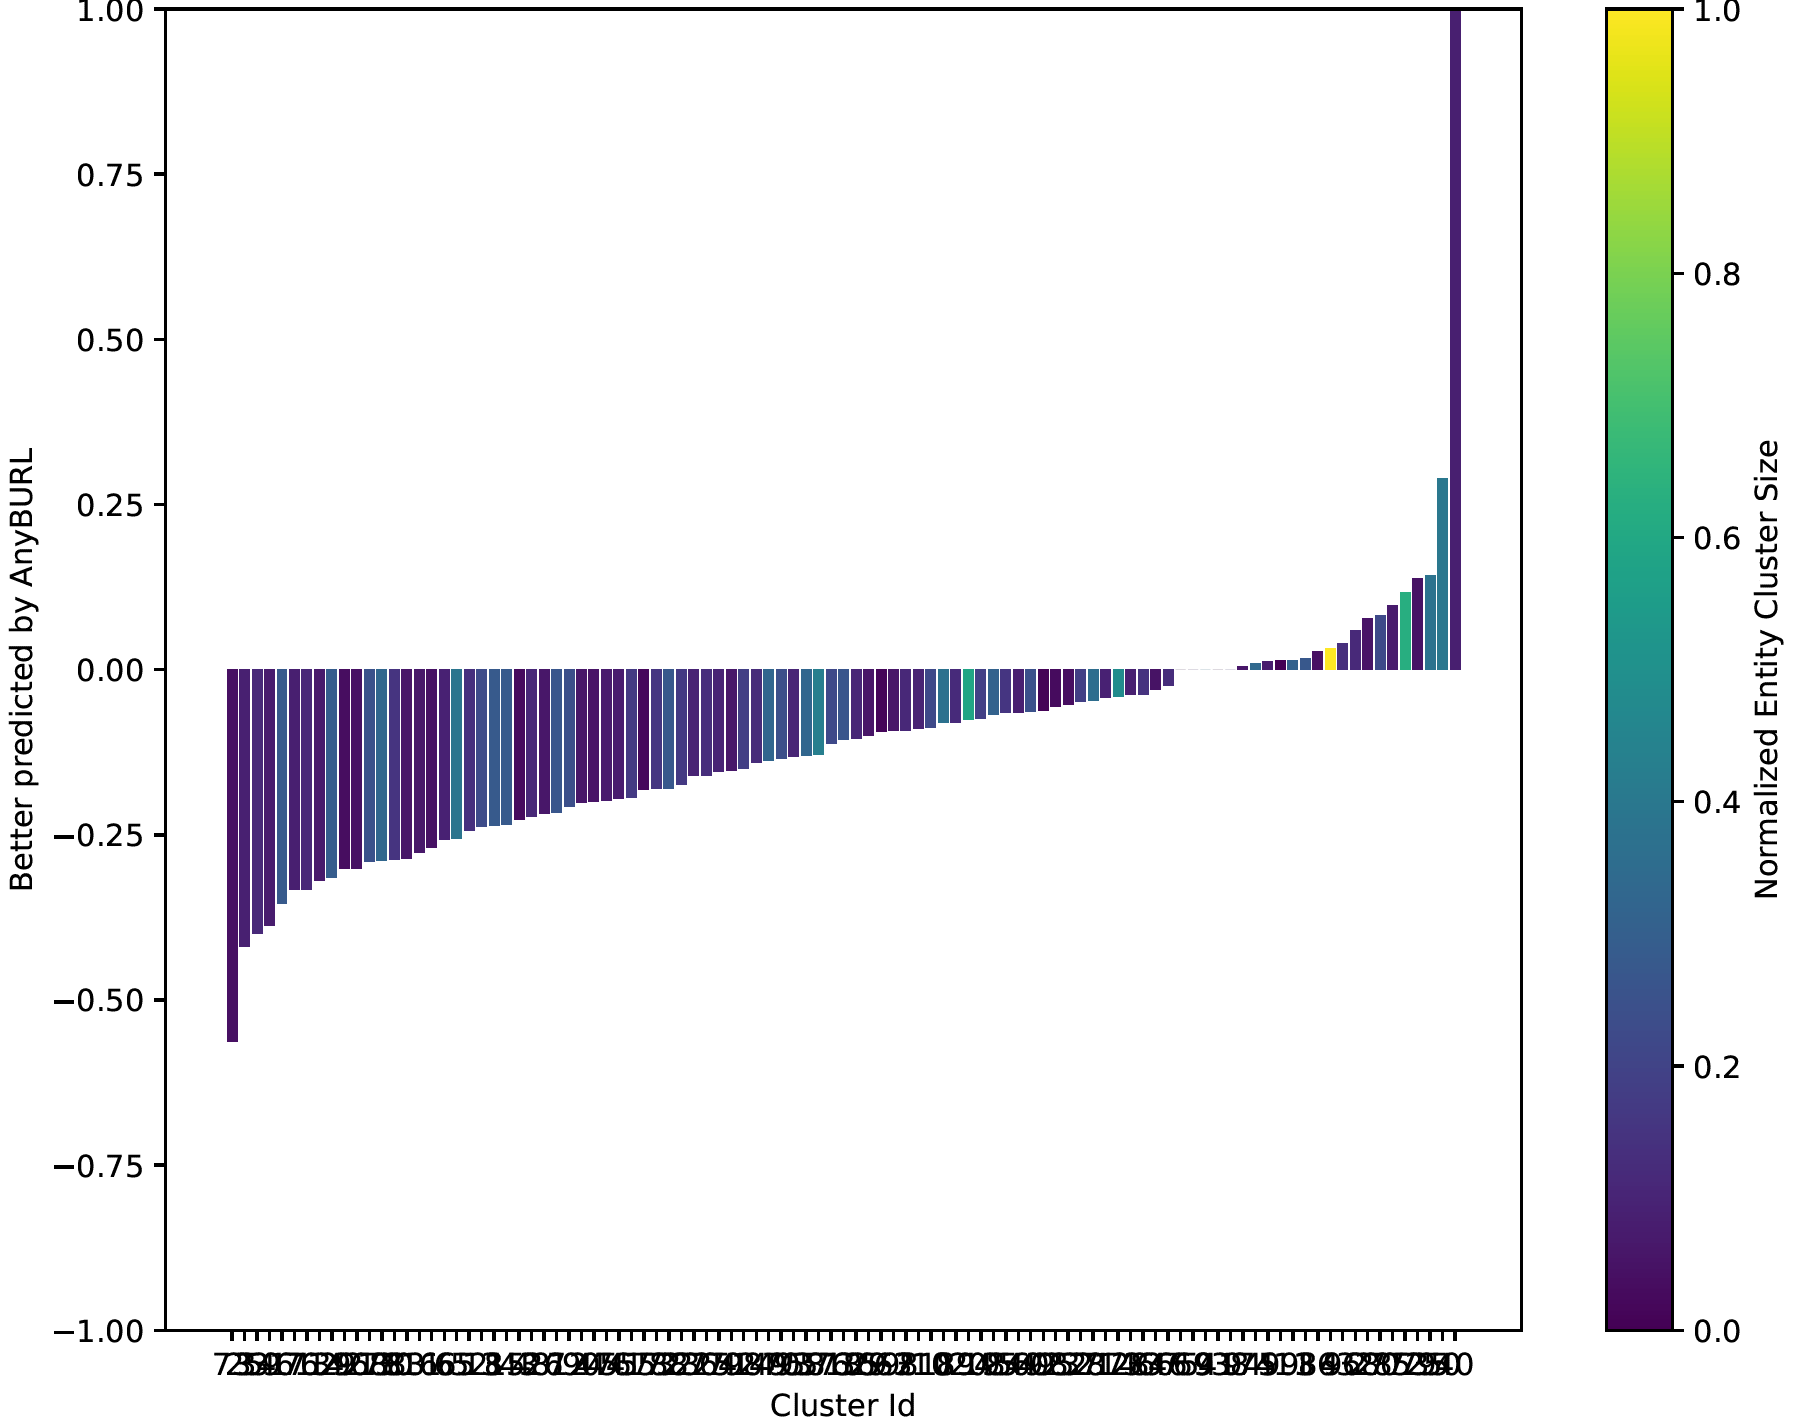
\includegraphics[width=0.7\textwidth]{images/tail_cluster_100_anyburl_conve_fb15k.PNG}
\caption{Comparison of AnyBURL and ConvE on FB15k-237 in regard to the existence of similar tail entities based on K-Means Clustering (k=100)}
\label{fig:tail_cluster_100_anyburl_conve_fb15k}
\end{figure}

\subsection{AnyBURL and RESCAL on FB15k-237}

\begin{figure}[H]
\centering
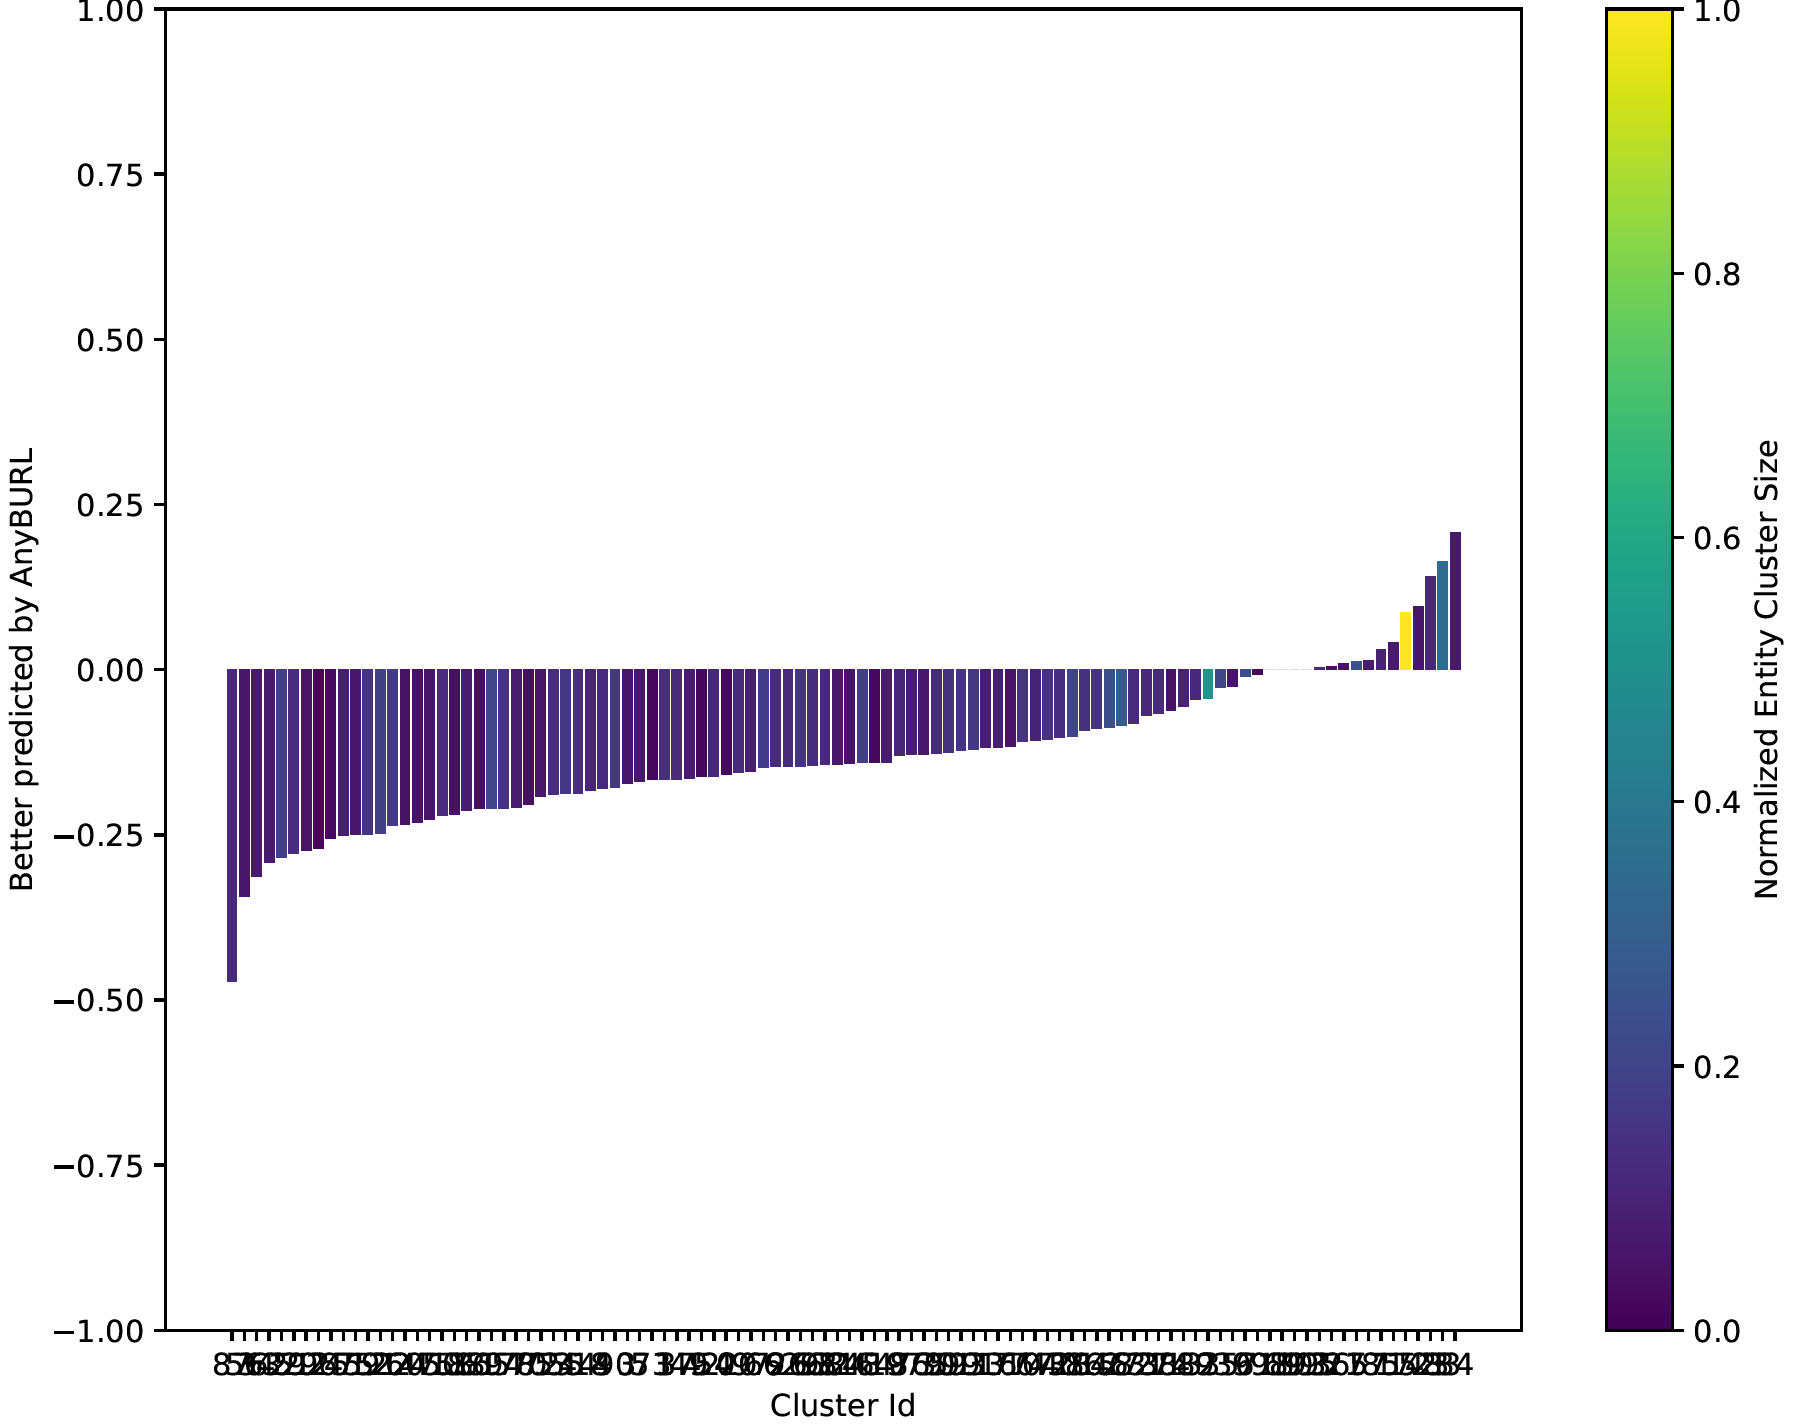
\includegraphics[width=0.7\textwidth]{images/head_cluster_100_anyburl_rescal_fb15k.PNG}
\caption{Comparison of AnyBURL and RESCAL on FB15k-237 in regard to the existence of similar head entities based on K-Means Clustering (k=100)}
\label{fig:head_cluster_100_anyburl_rescal_fb15k}
\end{figure}

\begin{figure}[H]
\centering
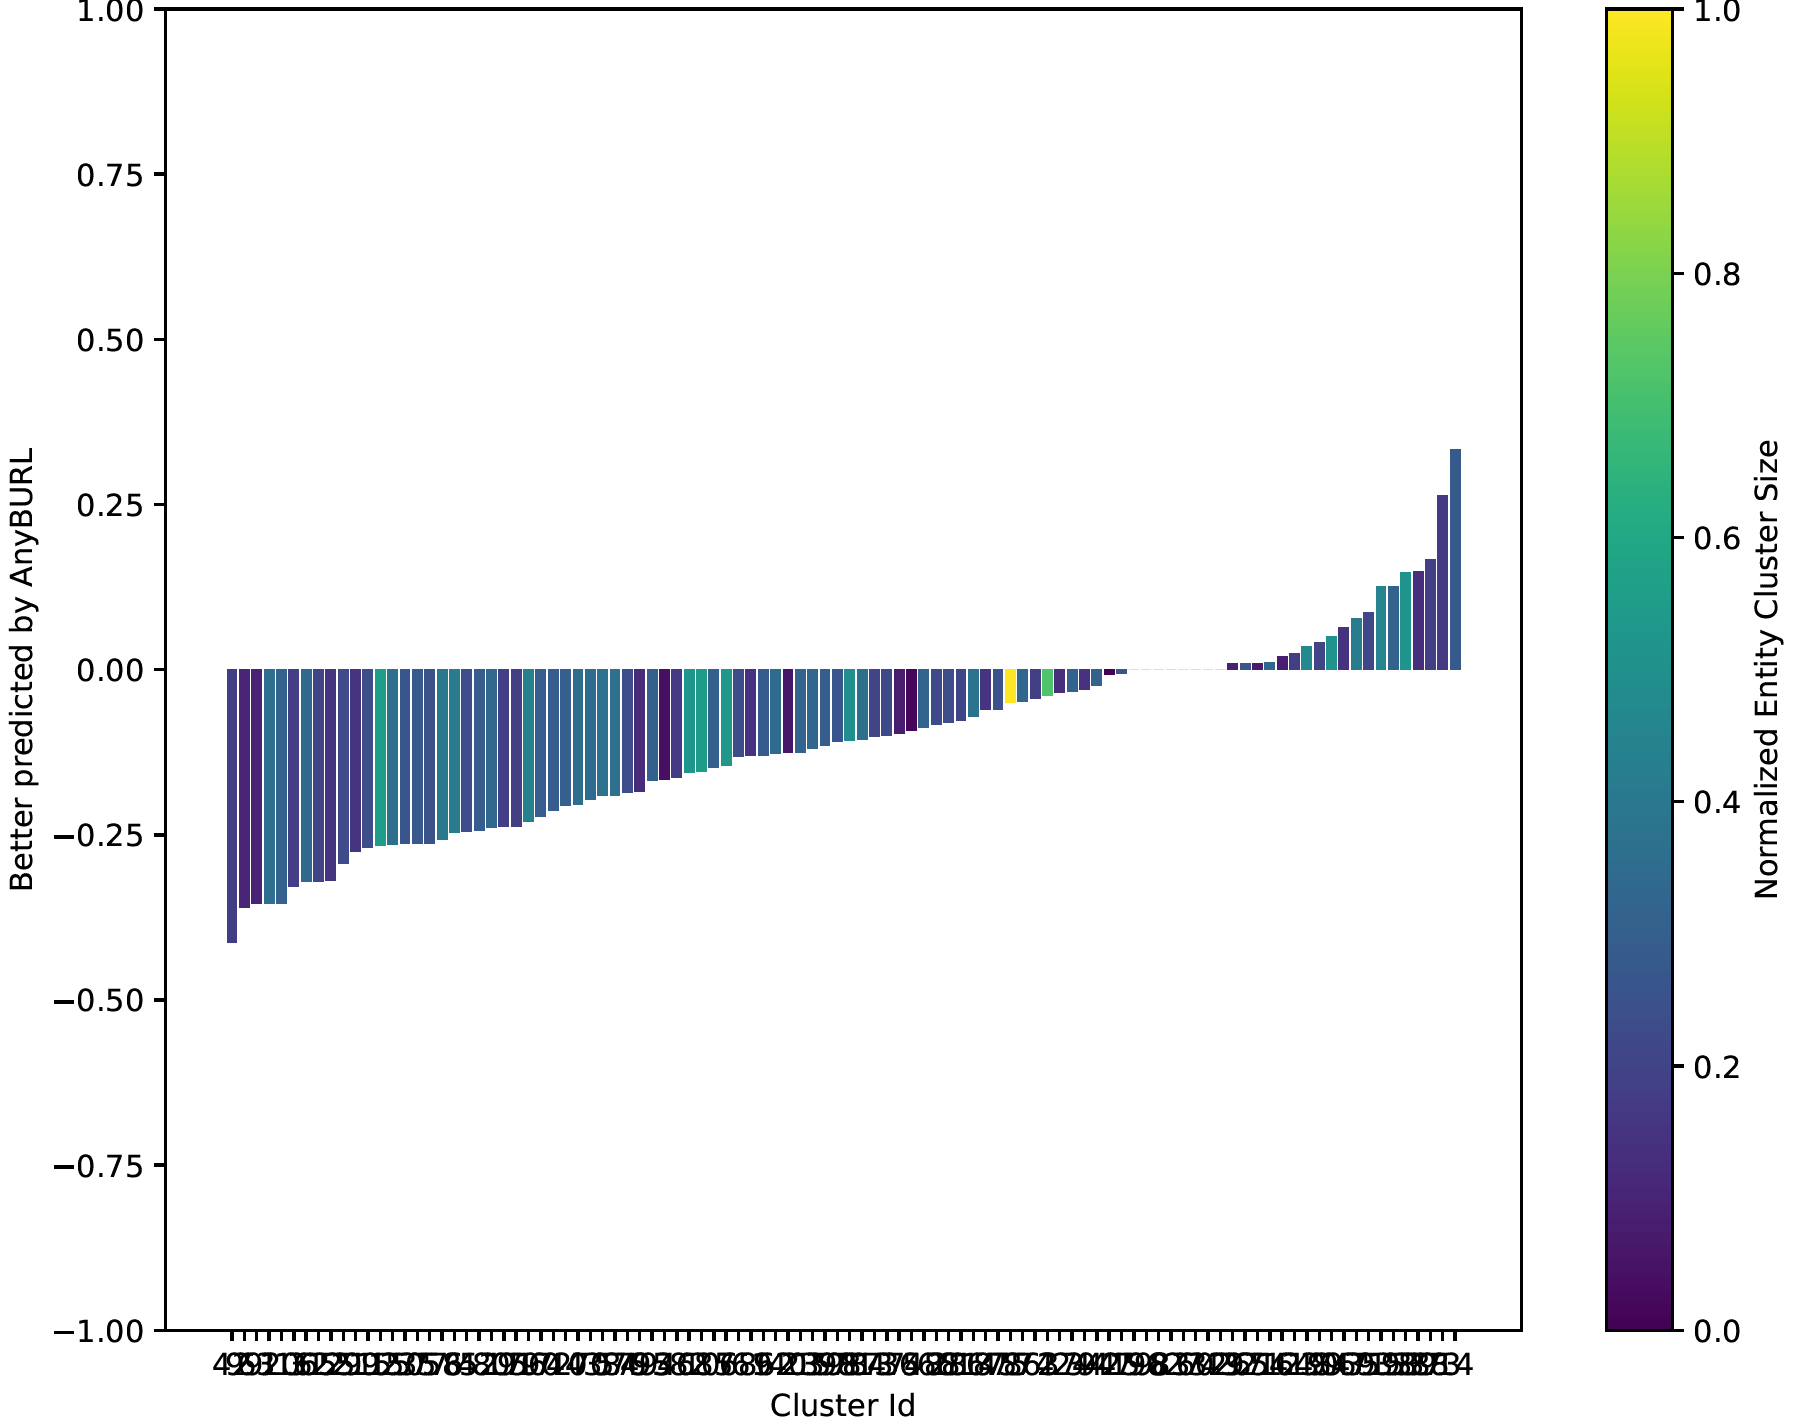
\includegraphics[width=0.7\textwidth]{images/tail_cluster_100_anyburl_rescal_fb15k.PNG}
\caption{Comparison of AnyBURL and RESCAL on FB15k-237 in regard to the existence of similar tail entities based on K-Means Clustering (k=100)}
\label{fig:tail_cluster_100_anyburl_rescal_fb15k}
\end{figure}

\subsection{AnyBURL and ComplEx on YAGO3-10}

\begin{figure}[H]
\centering
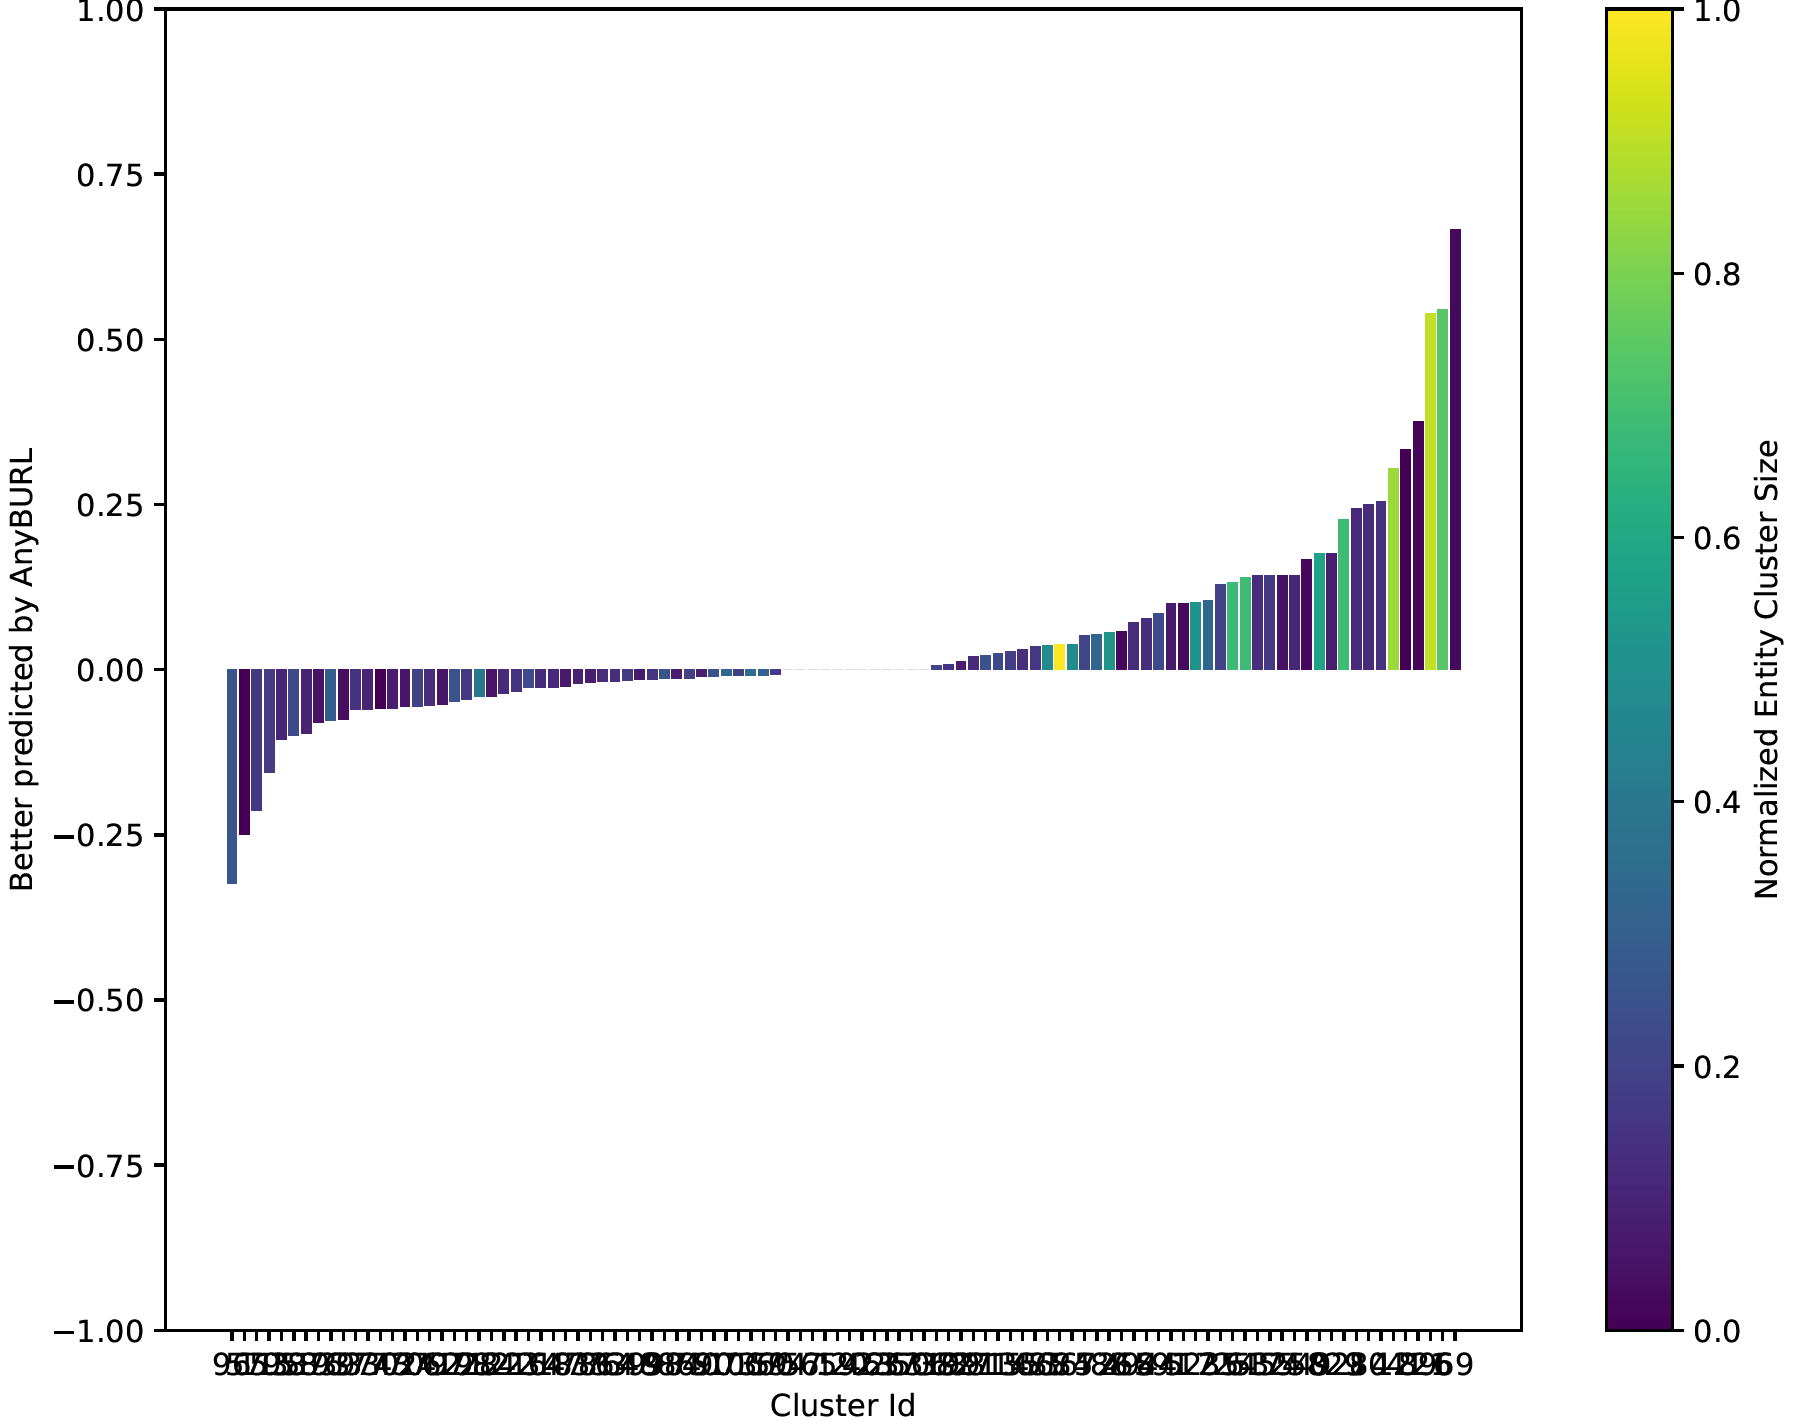
\includegraphics[width=0.7\textwidth]{images/head_cluster_100_anyburl_complex_yago.PNG}
\caption{Comparison of AnyBURL and ComplEx on YAGO3-10 in regard to the existence of similar head entities based on K-Means Clustering (k=100)}
\label{fig:head_cluster_100_anyburl_complex_yago}
\end{figure}
